\section{The board}\label{sec:board}

This section fixes the notation for the board and proves the elementary facts about its geometry on
which the whole argument rests: the number of lines, the fact that two cells determine at most one line,
the number of lines through a cell, and the group of symmetries that is used to store positions in a
canonical form. All of this is easily confirmed by a few lines of code, and every program of
\cref{sec:verification} does so; we give proofs by hand so that the main theorem depends on no computed
description of the board.

\subsection{Cells and lines}\label{ssec:lines}

The \emph{board} is $\Q=\{0,1,\dots,5\}^3$; its $216$ elements are the \emph{cells}. We write a cell as
$c=(c_1,c_2,c_3)$ or as $(x,y,z)$. Let $\rho$ denote the reversal $i\mapsto 5-i$ of $\{0,\dots,5\}$.

A \emph{parametrization} is a triple $f=(f_1,f_2,f_3)$ of maps $\{0,\dots,5\}\to\{0,\dots,5\}$ each of which
is a constant map, the identity, or $\rho$, and which are not all constant. A coordinate $i$ is
\emph{active} in $f$ if $f_i$ is not constant. The \emph{line} of $f$ is the set
\[
  \ell(f)=\{f(t) : 0\le t\le 5\},\qquad f(t)=(f_1(t),f_2(t),f_3(t)),
\]
and $\Lines$ denotes the set of all lines. Clearly $\ell(f\circ\rho)=\ell(f)$, where
$f\circ\rho=(f_1\circ\rho,f_2\circ\rho,f_3\circ\rho)$; note that $f\circ\rho$ has the same active coordinates
as $f$. A line with one, two or three active coordinates is called an \emph{axis line}, a \emph{face
diagonal} or a \emph{space diagonal}, respectively; by part~(a) of the following lemma this does not
depend on the parametrization.

\begin{lemma}[Geometry of the board]\label{lem:geometry}
\begin{enumerate}[label=\textup{(\alph*)}]
\item Every line consists of six distinct cells and has exactly two parametrizations, $f$ and $f\circ\rho$.
\item There are exactly $148$ lines: $108$ axis lines, $36$ face diagonals and $4$ space diagonals.
\item Two distinct cells lie on at most one line. Equivalently, two distinct lines have at most one cell in
      common.
\end{enumerate}
\end{lemma}

\begin{proof}
Let $f$ be a parametrization, let $t_1\ne t_2$, and put $p=f(t_1)$, $q=f(t_2)$. If $f_i$ is constant, then
$p_i=q_i$; if $i$ is active, then $f_i$ is injective and $p_i\ne q_i$. Hence
\begin{equation}\label{eq:active}
  \text{the active coordinates of $f$ are exactly the coordinates in which $p$ and $q$ differ.}
\end{equation}
Since at least one coordinate is active, $f$ is injective, so $\ell(f)$ has six cells.

Now let $p\ne q$ be two cells of a line $\ell$, and let $i_0$ be the smallest coordinate with
$p_{i_0}\ne q_{i_0}$. By \eqref{eq:active} the coordinate $i_0$ is active in every parametrization of $\ell$,
and exactly one of the two maps $f_{i_0}$, $f_{i_0}\circ\rho$ is the identity; so $\ell$ has a
parametrization $f$ with $f_{i_0}=\mathrm{id}$. We claim that such an $f$ is determined by $p$ and $q$.
Indeed, let $p=f(t_1)$. Then $t_1=f_{i_0}(t_1)=p_{i_0}$. If $p_i=q_i$, then $f_i$ is the constant map with
value $p_i$, by \eqref{eq:active}. If $p_i\ne q_i$, then $f_i\in\{\mathrm{id},\rho\}$ by \eqref{eq:active},
and $f_i(t_1)=p_i$ means that $p_i=t_1$ if $f_i=\mathrm{id}$ and $p_i=5-t_1$ if $f_i=\rho$. As
$t_1\ne 5-t_1$ (because $5$ is odd), these two cases exclude each other, so $f_i$ is determined by $p_i$
and $t_1=p_{i_0}$.

(c) If $p\ne q$ lie on two lines $\ell$ and $\ell'$, then both lines have a parametrization whose
$i_0$-th component is the identity, where $i_0$ depends only on $p$ and $q$; by the claim the two
parametrizations coincide, hence $\ell=\ell'$. The second formulation is equivalent to the first.

(a) Let $\ell(f)=\ell(f')$, choose two cells $p\ne q$ of this line and define $i_0$ as above. One of
$f,f\circ\rho$ and one of $f',f'\circ\rho$ has the identity as its $i_0$-th component, and these two
parametrizations coincide by the claim. Hence $f'\in\{f,f\circ\rho\}$. Finally $f\circ\rho\ne f$, since an
active component is changed.

(b) By (a) the number of lines is half the number of parametrizations. A parametrization with a given set
of $j$ active coordinates is obtained by choosing $\mathrm{id}$ or $\rho$ for each active coordinate and one
of six constants for each of the others, in $2^j6^{3-j}$ ways. This gives $3\cdot 2\cdot 36/2=108$ axis
lines, $3\cdot 4\cdot 6/2=36$ face diagonals and $8/2=4$ space diagonals; in total
$(8^3-6^3)/2=148$ lines.
\end{proof}

Part (c) is used constantly, mostly in the form $|a\cap b|\le 1$ for distinct lines $a,b$. Two cells that
lie on a common line are called \emph{collinear}. The proof gives a test for collinearity which we record
for later use.

\begin{corollary}[Collinearity]\label{cor:collinear}
Two distinct cells $p,q$ are collinear if and only if there are numbers $t_1\ne t_2$ such that
$(p_i,q_i)\in\{(t_1,t_2),(5-t_1,5-t_2)\}$ for every coordinate $i$ with $p_i\ne q_i$. The line through
$p$ and $q$ is then an axis line, a face diagonal or a space diagonal according as $p$ and $q$ differ in
one, two or three coordinates.
\end{corollary}

\begin{proof}
If $p=f(t_1)$ and $q=f(t_2)$ for a parametrization $f$, then $t_1\ne t_2$, and for a coordinate $i$ with
$p_i\ne q_i$ we have $f_i=\mathrm{id}$ or $f_i=\rho$ by \eqref{eq:active}, that is,
$(p_i,q_i)=(t_1,t_2)$ or $(p_i,q_i)=(5-t_1,5-t_2)$. Conversely, given $t_1\ne t_2$ with the stated property,
let $f_i$ be the constant $p_i$ if $p_i=q_i$, the identity if $(p_i,q_i)=(t_1,t_2)$, and $\rho$ otherwise;
then $f$ is a parametrization (as $p\ne q$) with $f(t_1)=p$ and $f(t_2)=q$. The last statement is
\eqref{eq:active}.
\end{proof}

\subsection{Lines through a cell; busy cells}\label{ssec:busy}

For $i\in\{0,\dots,5\}$ let $\lambda(i)=\min(i,5-i)\in\{0,1,2\}$ be the \emph{level} of $i$; thus
$\lambda(i)=\lambda(j)$ if and only if $j\in\{i,5-i\}$.

\begin{lemma}[Lines through a cell]\label{lem:degree}
Let $c=(c_1,c_2,c_3)$ be a cell and let $A$ be a non-empty set of coordinates. There is a line through $c$
whose set of active coordinates is $A$ if and only if the levels $\lambda(c_i)$, $i\in A$, are all equal;
in this case there is exactly one such line. Consequently $c$ lies on exactly three axis lines, on
exactly one face diagonal for every pair $i<j$ with $\lambda(c_i)=\lambda(c_j)$, and on exactly one space
diagonal if $\lambda(c_1)=\lambda(c_2)=\lambda(c_3)$, and on no other line. The number of lines through $c$
is $7$, $4$ or $3$ according as the levels $\lambda(c_1),\lambda(c_2),\lambda(c_3)$ take one, two or three
distinct values, and there are $24$, $144$ and $48$ cells of these three kinds.
\end{lemma}

\begin{proof}
Let $i_0=\min A$. By \cref{lem:geometry}\,(a) a line with active set $A$ has exactly one parametrization
$f$ with $f_{i_0}=\mathrm{id}$, and $c=f(t)$ holds for some $t$ if and only if it holds for $t=c_{i_0}$.
This requires $f_i$ to be the constant $c_i$ for $i\notin A$, and for $i\in A$ it requires
$f_i=\mathrm{id}$ and $c_i=c_{i_0}$, or $f_i=\rho$ and $c_i=5-c_{i_0}$. Since $c_{i_0}\ne 5-c_{i_0}$, such
an $f$ exists if and only if $c_i\in\{c_{i_0},5-c_{i_0}\}$ for all $i\in A$, and then it is unique. This
proves the first statement, and the list of lines through $c$ follows by taking $|A|=1,2,3$. If the three
levels are equal, $c$ lies on $3+3+1=7$ lines; if exactly two are equal, on $3+1=4$; if they are distinct,
on $3$. Each triple of levels belongs to $2^3=8$ cells; $3$ triples are constant, $6$ consist of distinct
levels, and $27-3-6=18$ contain exactly two equal levels, which gives $24$, $48$ and $144$ cells.
\end{proof}

As a check, counting the incident pairs (cell, line) in two ways gives
$24\cdot 7+144\cdot 4+48\cdot 3=888=148\cdot 6$.

\begin{definition}[Busy cells, antipodes]\label{def:busy}
A cell $(x,y,z)$ is \emph{busy} if $\lambda(x)=\lambda(y)=\lambda(z)$; this common value is its \emph{level}.
The set of the $24$ busy cells is denoted by $\Busy$. The \emph{antipode} of a cell $c=(x,y,z)$ is
$\antip{c}=(5-x,5-y,5-z)$.
\end{definition}

By \cref{lem:degree} the busy cells are exactly the cells that lie on seven lines, and exactly the cells
that lie on a space diagonal; every other cell lies on three or four lines. A stone on a busy cell
therefore meets more lines than any other stone, which is why these cells play the main role in the
opening of the game. The eight busy cells of level $j$ are the corners $\{j,5-j\}^3$ of a cube; see
\cref{fig:busy}.

\begin{figure}[t]
\centering
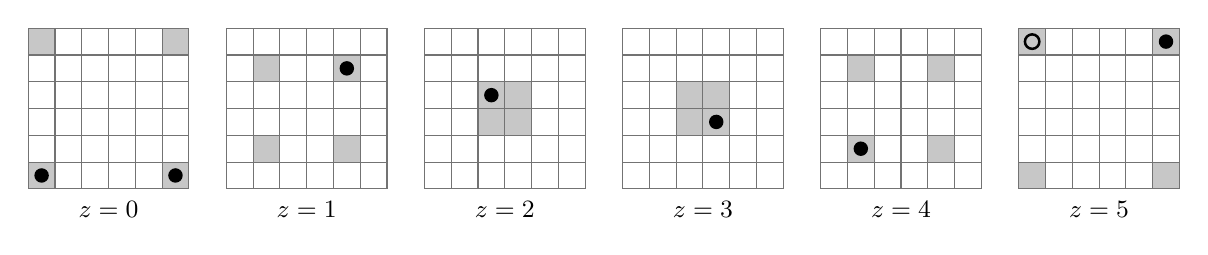
\begin{tikzpicture}[scale=0.34]
\foreach \z in {0,...,5} {
  \begin{scope}[shift={(7.4*\z,0)}]
    \pgfmathtruncatemacro{\w}{5-\z}
    \foreach \x in {\z,\w} { \foreach \y in {\z,\w} { \fill[black!22] (\x,\y) rectangle ++(1,1); } }
    \draw[step=1,black!55,thin] (0,0) grid (6,6);
    \node[below] at (3,-0.1) {\small $z=\z$};
  \end{scope}
}
\foreach \x/\y/\z in {0/0/0,5/0/0,4/4/1,2/3/2,3/2/3,1/1/4,5/5/5}
  { \fill (7.4*\z+\x+0.5,\y+0.5) circle (0.27); }
\draw[line width=0.9pt] (7.4*5+0+0.5,5+0.5) circle (0.27);
\end{tikzpicture}
\caption{The six layers $z=0,\dots,5$ of the board; in each layer $x$ increases to the right and $y$
upwards. Shaded: the $24$ busy cells. Dots: the seven cells of the set $\Tseven$ of \cref{ex:T7};
the set $\Teight$ of \cref{ex:T8} contains in addition the cell $(0,5,5)$ marked by a ring.}
\label{fig:busy}
\end{figure}

\begin{lemma}[Busy cells and lines]\label{lem:busy}
\begin{enumerate}[label=\textup{(\alph*)}]
\item A space diagonal consists of six busy cells, two of each level, and contains the antipode of each
      of its cells. The four space diagonals are pairwise disjoint and partition $\Busy$.
\item Every face diagonal contains exactly two busy cells. An axis line contains two busy cells or none;
      exactly $72$ axis lines contain none, namely those whose two constant coordinates have different
      levels.
\item Two distinct busy cells are collinear if and only if they have the same level or lie on the same
      space diagonal.
\end{enumerate}
\end{lemma}

\begin{proof}
(a) Let $f$ be a parametrization with three active coordinates. The coordinates of $f(t)$ are $t$ or
$5-t$, so $f(t)$ is busy of level $\lambda(t)$, and each level occurs for two values of $t$. For each $i$
we have $5-f_i(t)=f_i(5-t)$, both for $f_i=\mathrm{id}$ and for $f_i=\rho$; hence
$\antip{f(t)}=f(5-t)\in\ell(f)$. By \cref{lem:degree} every busy cell lies on exactly one space diagonal.

(b) On a face diagonal with constant coordinate $v$ the cell with parameter $t$ has the levels
$\lambda(t),\lambda(t),\lambda(v)$ and is busy if and only if $t\in\{v,5-v\}$. On an axis line with constant
coordinates $v,w$ the cell with parameter $t$ is busy if and only if $\lambda(t)=\lambda(v)=\lambda(w)$;
this holds for two values of $t$ if $\lambda(v)=\lambda(w)$ and for none otherwise. For each of the three
directions there are $36-3\cdot 4=24$ pairs $(v,w)$ with $\lambda(v)\ne\lambda(w)$.

(c) Let $p\ne q$ be busy. If both have level $j$, then $(p_i,q_i)\in\{(j,5-j),(5-j,j)\}$ whenever
$p_i\ne q_i$, and $p,q$ are collinear by \cref{cor:collinear} with $(t_1,t_2)=(j,5-j)$. If their levels are
different, then $p_i\ne q_i$ for every $i$, so by \cref{cor:collinear} a line through $p$ and $q$ is a
space diagonal.
\end{proof}

\subsection{Symmetries}\label{ssec:group}

Let $H$ be the group of all permutations $s$ of $\{0,\dots,5\}$ that commute with $\rho$, that is,
$s(5-i)=5-s(i)$ for all $i$. Such an $s$ permutes the three pairs $\{0,5\}$, $\{1,4\}$, $\{2,3\}$ and is
determined by $s(0),s(1),s(2)$, for which there are $6$, $4$ and $2$ possibilities; hence $|H|=48$. We
consider three kinds of maps $\Q\to\Q$:
\begin{itemize}
\item for a permutation $\pi$ of $\{1,2,3\}$, the map $\Pi_\pi$ that moves the $i$-th coordinate to
      position $\pi(i)$: $(\Pi_\pi c)_{\pi(i)}=c_i$;
\item for a set $r\subseteq\{1,2,3\}$, the map $\mathrm{P}_r$ that replaces $c_i$ by $5-c_i$ for every
      $i\in r$;
\item for $s\in H$, the map $\Sigma_s$ that applies $s$ to every coordinate:
      $\Sigma_s(c)=(s(c_1),s(c_2),s(c_3))$.
\end{itemize}
Let
\[
  \G=\{\Sigma_s\circ\mathrm{P}_r\circ\Pi_\pi : s\in H,\ r\subseteq\{1,2,3\},\ \pi\in S_3\}.
\]
The $48$ maps $\mathrm{P}_r\circ\Pi_\pi$ are the symmetries of the cube. The maps $\Sigma_s$ with
$s\notin\{\mathrm{id},\rho\}$ are not isometries: they permute and reverse the three pairs of layers
$\{i,5-i\}$ in all three directions simultaneously. For a map $g$ and a set $Y$ of cells we write
$gY=\{g(c):c\in Y\}$, and $gS=\{gl : l\in S\}$ for a set $S$ of lines.

\begin{lemma}[The group $\G$]\label{lem:group}
\begin{enumerate}[label=\textup{(\alph*)}]
\item Every $g\in\G$ is a bijection of $\Q$ that maps every line onto a line of the same kind (axis line,
      face diagonal, space diagonal). Hence $g$ induces a permutation $l\mapsto gl$ of $\Lines$.
\item $\G$ is closed under composition and under inversion, that is, $\G$ is a group.
\item $|\G|=1{,}152$.
\item Every $g\in\G$ maps $\Busy$ onto $\Busy$ and commutes with the antipodal map:
      $g(\antip{c})=\antip{g(c)}$ for every cell $c$.
\end{enumerate}
\end{lemma}

\begin{proof}
(a) The maps $\Pi_\pi$, $\mathrm{P}_r$, $\Sigma_s$ are bijections with inverses $\Pi_{\pi^{-1}}$,
$\mathrm{P}_r$, $\Sigma_{s^{-1}}$. Let $f$ be a parametrization. Then $\Pi_\pi(\ell(f))=\ell(f')$, where
$f'$ arises from $f$ by permuting the components. Next, $\mathrm{P}_r(\ell(f))=\ell(f')$ with
$f'_i=\rho\circ f_i$ for $i\in r$ and $f'_i=f_i$ otherwise; here $\rho\circ f_i$ is constant, $\rho$ or the
identity if $f_i$ is constant, the identity or $\rho$, respectively. Finally,
$\Sigma_s(\ell(f))=\{(s f_1(t),s f_2(t),s f_3(t)):0\le t\le 5\}$. With the new parameter $t'=s(t)$, which
runs through $\{0,\dots,5\}$ as $t$ does, we have $s(f_i(t))=s(v)$ if $f_i$ is the constant $v$,
$s(f_i(t))=t'$ if $f_i=\mathrm{id}$, and $s(f_i(t))=s(5-t)=5-t'$ if $f_i=\rho$; so
$\Sigma_s(\ell(f))=\ell(f')$, where $f'$ has the same components as $f$ except that each constant $v$ is
replaced by $s(v)$. In all three cases $f'$ is a parametrization with as many active coordinates as $f$.
Thus each of the three kinds of maps, and therefore each $g\in\G$, maps lines onto lines of the same kind.
Being injective on cells, $g$ induces an injective map of the finite set $\Lines$ into itself, that is, a
permutation.

(b) Each of the sets $\G_\Sigma=\{\Sigma_s\}$, $\G_{\mathrm P}=\{\mathrm{P}_r\}$, $\G_\Pi=\{\Pi_\pi\}$ is a
subgroup of the symmetric group of $\Q$, because $\Sigma_s\Sigma_{s'}=\Sigma_{ss'}$,
$\mathrm{P}_r\mathrm{P}_{r'}=\mathrm{P}_{r\triangle r'}$ and $\Pi_\pi\Pi_{\pi'}=\Pi_{\pi\pi'}$. Moreover
\[
  \Sigma_s\Pi_\pi=\Pi_\pi\Sigma_s,\qquad \Sigma_s\mathrm{P}_r=\mathrm{P}_r\Sigma_s,\qquad
  \Pi_\pi\mathrm{P}_r\Pi_\pi^{-1}=\mathrm{P}_{\pi(r)}:
\]
the first relation is obvious, the second holds because $s\rho=\rho s$, and the third says that reversing
the coordinates in $r$ and then moving coordinate $i$ to position $\pi(i)$ is the same as first moving
the coordinates and then reversing those in $\pi(r)$. By the third relation
$K=\G_{\mathrm P}\G_\Pi=\G_\Pi\G_{\mathrm P}$ is a subgroup; by the first two, every element of $\G_\Sigma$
commutes with every element of $K$. Hence $\G=\G_\Sigma K=K\G_\Sigma$ is closed under composition,
$(\sigma\kappa)(\sigma'\kappa')=(\sigma\sigma')(\kappa\kappa')$, and under inversion,
$(\sigma\kappa)^{-1}=\sigma^{-1}\kappa^{-1}$ for $\sigma,\sigma'\in\G_\Sigma$ and $\kappa,\kappa'\in K$.

(c) We have $|\G_\Sigma|=48$. A map $\Pi_\pi$ fixes the cell $(0,0,0)$, while $\mathrm{P}_r(0,0,0)$ has the
entry $5$ exactly in the positions of $r$; hence $\G_{\mathrm P}\cap\G_\Pi=\{\mathrm{id}\}$ and
$|K|=8\cdot 6=48$. Suppose that $\Sigma_s=\mathrm{P}_r\Pi_\pi$, and evaluate both sides at the cells
$(i,i,i)$: the left side is $(s(i),s(i),s(i))$, and the right side has the entry $5-i$ in the positions of
$r$ and the entry $i$ elsewhere. As $i\ne 5-i$, either $r=\emptyset$ and $s=\mathrm{id}$, or $r=\{1,2,3\}$
and $s=\rho$; in both cases $\Sigma_s=\mathrm{P}_r$, so $\Pi_\pi=\mathrm{id}$. Hence
$\G_\Sigma\cap K=\{\mathrm{id},\Sigma_\rho\}$, where $\Sigma_\rho=\mathrm{P}_{\{1,2,3\}}$, and
$|\G|=|\G_\Sigma|\,|K|/|\G_\Sigma\cap K|=48\cdot 48/2=1{,}152$.

(d) By (a), $g$ permutes the space diagonals, and $\Busy$ is their union (\cref{lem:busy}\,(a)). The
antipodal map is $\Sigma_\rho=\mathrm{P}_{\{1,2,3\}}$. It commutes with every $\Sigma_s$ and every
$\mathrm{P}_r$, and with every $\Pi_\pi$ by the third relation above with $r=\{1,2,3\}$.
\end{proof}

The triples $(s,r,\pi)$ thus describe each map of $\G$ exactly twice. The group property in (b) is what
makes canonical forms well behaved (\cref{lem:canon} below).

\subsection{Stones and live lines}\label{ssec:live}

Throughout the paper $B$ denotes a set of cells occupied by \Breaker{} and $X$ a set of cells occupied by
\Maker{} (their \emph{stones}), with $B\cap X=\emptyset$. For a set $Y$ of cells and a cell $c$ we write
$Y+c$ for $Y\cup\{c\}$. A line is \emph{live} (with respect to $B$) if it contains no cell of $B$, and
\emph{dead} otherwise; only live lines can still be completed by \Maker. We write
\[
  \live{B}=\{l\in\Lines : l\cap B=\emptyset\},\qquad \N(S)=\bigcup_{l\in S}l\quad(S\subseteq\Lines)
\]
for the set of live lines and for the set of cells covered by a set $S$ of lines. If $S\subseteq\live{B}$,
then $\N(S)\cap B=\emptyset$. For $g\in\G$ it follows from \cref{lem:group}\,(a) that
\begin{equation}\label{eq:inv-basic}
  \live{gB}=g\,\live{B},\qquad \N(gS)=g\,\N(S),\qquad |gl\cap gY|=|l\cap Y|
\end{equation}
for all sets $B,Y$ of cells, all lines $l$ and all sets $S$ of lines. All notions introduced in
\cref{sec:pairing,sec:leaf} are defined in terms of cells, lines, membership and cardinalities only, and
are therefore invariant under $\G$; the precise statement is \cref{lem:invariance} at the end of
\cref{sec:leaf}.

\subsection{Canonical forms}\label{ssec:canon}

The strategy constructed in this paper is stored as a table of positions, and positions that differ by a
map of $\G$ are stored only once. To this end we order the cells lexicographically, $(x,y,z)<(x',y',z')$
if $x<x'$, or $x=x'$ and $y<y'$, or $x=x'$, $y=y'$ and $z<z'$; equivalently, by the number $36x+6y+z$,
which serves as the name of the cell in the files of \cref{sec:formats}. For two different sets $A,A'$ of
cells we put
\[
  A<A' \quad:\Longleftrightarrow\quad \text{the smallest cell of the symmetric difference }A\triangle A'
  \text{ belongs to }A .
\]
This is a total order on the sets of cells (it is the lexicographic order of the indicator vectors, with
the entry $1$ preceding the entry $0$). For sets of equal size it is the lexicographic order of the
increasingly sorted lists of cells: if $a_1<\dots<a_n$ and $a'_1<\dots<a'_n$ first differ in position $j$
and $a_j<a'_j$, then $a_j$ is the smallest cell of $A\triangle A'$. Pairs of sets are ordered
lexicographically: $(A_1,A_2)<(A'_1,A'_2)$ if $A_1<A'_1$, or $A_1=A'_1$ and $A_2<A'_2$.

\begin{definition}[Canonical form]\label{def:canon}
For two sets $B,F$ of cells, the \emph{canonical form} of the pair $(B,F)$ is
\[
  \canon(B,F)=\min\{(gB,gF) : g\in\G\},
\]
the minimum being taken with respect to the order just defined (the sets $gB$ are compared first). The
pair $(B,F)$ is \emph{canonical} if $\canon(B,F)=(B,F)$.
\end{definition}

In \cref{sec:game} the set $B$ will be the set of \Breaker's stones and $F$ a set of stones of \Maker; a
state of the game there also carries a round number, which is not affected by $\G$.

\begin{lemma}[Canonical forms and translation of moves]\label{lem:canon}
Let $B,F$ be sets of cells.
\begin{enumerate}[label=\textup{(\alph*)}]
\item $\canon(hB,hF)=\canon(B,F)$ for every $h\in\G$.
\item Let $g\in\G$ be any map with $(gB,gF)=\canon(B,F)=:(B^{\mathrm c},F^{\mathrm c})$, let
      $m^{\mathrm c}$ be a cell and $m=g^{-1}(m^{\mathrm c})$. Then $m\notin B\cup F$ if and only if
      $m^{\mathrm c}\notin B^{\mathrm c}\cup F^{\mathrm c}$, and
      \[
        g(B+m)=B^{\mathrm c}+m^{\mathrm c},\qquad g(F+m)=F^{\mathrm c}+m^{\mathrm c};
      \]
      consequently $\canon(B+m,F)=\canon(B^{\mathrm c}+m^{\mathrm c},F^{\mathrm c})$ and
      $\canon(B,F+m)=\canon(B^{\mathrm c},F^{\mathrm c}+m^{\mathrm c})$.
\item If $g,g'\in\G$ both satisfy $(gB,gF)=(g'B,g'F)=\canon(B,F)$, then $h=g'^{-1}g$ satisfies $hB=B$
      and $hF=F$, and $g'^{-1}(m^{\mathrm c})=h\bigl(g^{-1}(m^{\mathrm c})\bigr)$ for every cell
      $m^{\mathrm c}$.
\end{enumerate}
\end{lemma}

\begin{proof}
(a) Since $\G$ is a group (\cref{lem:group}\,(b)), $g\mapsto gh$ is a bijection of $\G$, so the sets
$\{(ghB,ghF):g\in\G\}$ and $\{(gB,gF):g\in\G\}$ coincide. (b) The displayed equations and the equivalence
hold because $g$ is a bijection with $g(m)=m^{\mathrm c}$; the last statement follows from them by (a),
applied to the pairs $(B+m,F)$ and $(B,F+m)$ with $h=g$. (c) is clear, using again that $\G$ is a group.
\end{proof}

Part (b) is the form in which the lemma is used: the table of \cref{sec:game} lists, for a canonical
pair $(B^{\mathrm c},F^{\mathrm c})$, a cell $m^{\mathrm c}$, and in a position described by $(B,F)$ the
move actually played is $m=g^{-1}(m^{\mathrm c})$. Since every property of positions that matters is
invariant under $\G$, the move $m$ is as good in $(B,F)$ as $m^{\mathrm c}$ is in
$(B^{\mathrm c},F^{\mathrm c})$, and the successor positions have the same canonical forms. If the
canonical form is attained by several maps $g$, the resulting moves differ by a symmetry of the pair
$(B,F)$, by (c); the statement (b) holds for each of them and never uses that $g$ is unique. Part (a)
guarantees that it does not matter whether canonical forms are computed from the real position or from a
position that has already been transformed, which is what the different programs of
\cref{sec:verification} do.

\subsection{The full automorphism group}\label{ssec:aut}

An \emph{automorphism} of the board is a bijection of $\Q$ that maps every line onto a line. By
\cref{lem:group} every element of $\G$ is an automorphism. The proof of the main theorem uses nothing
more, but it is natural to ask whether $\G$ misses any symmetry.

\begin{fact}[The full automorphism group; not used in the proof of \cref{thm:main}]\label{fact:aut}
The automorphism group of the incidence structure $(\Q,\Lines)$ has order $1{,}152$; hence it is equal
to~$\G$.

\established the program \fn{autgroup.cpp} in the directory \fn{logs/canon/} of the
project repository (output \fn{autgroup.log}; see \cref{ssec:artifact}), a
search by individualization and color refinement on the incidence graph with $216+148$ vertices. It
finds a base consisting of three lines and three cells; the orbit of each base point under the pointwise
stabilizer of the preceding ones has $4$, $3$, $2$, $6$, $4$, $2$ elements, respectively, so that the
group has order $4\cdot3\cdot2\cdot6\cdot4\cdot2=1{,}152$.
\end{fact}

For the $4\times4\times4$ board the automorphism group, which has order $192$, was determined by
Silver~\cite{Silver1967}, and the automorphism groups of the boards $n^d$ in general were characterized
by Dvo\v{r}\'ak and Valla~\cite{DvorakValla2021}. We did not rely on these results:
\cref{fact:aut} is a direct computation for the present board.

\begin{table}[tb]
\centering\small
\begin{tabular}{@{}lp{0.74\textwidth}@{}}
\toprule
symbol & meaning \\
\midrule
$\Q$, $\Lines$ & the $216$ cells and the $148$ lines (\cref{ssec:lines}) \\
$\lambda(i)$ & level $\min(i,5-i)$ of a coordinate value \\
$\Busy$, $\antip{c}$ & the $24$ busy cells; the antipode of the cell $c$ (\cref{def:busy}) \\
$\G$ & the group of $1{,}152$ symmetries (\cref{lem:group}) \\
$B$, $X$, $F$ & \Breaker's stones, \Maker's stones, the revealed stones of \Maker{} ($F\subseteq X$) \\
$Y+c$ & $Y\cup\{c\}$ \\
$\live{B}$ & the live lines, i.e.\ the lines without a cell of $B$ \\
$\N(S)$ & the union of the lines in $S$ \\
$\canon(B,F)$ & canonical form of a pair of sets (\cref{def:canon}) \\
$\dfc_X(S)$, $\slack(B)$ & deficiency $2|S|-|\N(S)\setminus X|$; slack $216-|B|-2|\live{B}|$ (\cref{sec:pairing}) \\
$\sur_F(S)$, $\Phi(B,F)$ & surplus $|\N(S)\setminus F|-2|S|$; least surplus of an $F$-connected set of
      at least three live lines (\cref{sec:leaf}) \\
$\mu(U)$ & least surplus of a set of live lines containing $U$ (\cref{ssec:deciding}) \\
$\CC$, $\CPhi$, $\LEAF$ & the certificates of \cref{def:C,def:leaf} \\
\bottomrule
\end{tabular}
\caption{Notation introduced in \cref{sec:board,sec:pairing,sec:leaf}.}
\label{tab:notation}
\end{table}
